\documentclass[fleqn]{article}

\usepackage{mydefs}
\usepackage{notes}
\usepackage{url}
\usepackage{graphicx}
\usepackage{subfig}
\usepackage{hyperref}

\begin{document}
\lecture{Reinforcement Learning Project}{Residual Algorithms: Reinforcement Learning with function approximation}{Srikanth Grandhe}

\section*{Introduction}
Residual Algorithms \footnote{www.leemon.com/papers/1995b.pdf} are a family of algorithms that provide guarentees of convergence and try to arrive to the convergence point faster than traditional algorithms that ensure these guarentees. This algorithm is obtained by trying to compute gradients that force the objective function to move in a non-increasing manner ensuring that the agent does not diverge. This is done by finding a sweet spot between two class of algorithms namely the direct algorithms and the residual gradient algorithms.

Some of the popular direct algorithms are Q-Learning and SARSA which arrive at the solution at good speed but lack the desired convergence properties. Whereas the other class of algorithms ie. the Residual Gradient Algorithms ensure the the convergence properties but arrive at the solution at a slower pace.

Direct Algorithm update equation:
\begin{equation}
w = w + \alpha * \delta * (\frac{\partial V(S_t)}{\partial w} )
\end{equation}

Residual Gradient update equation:
\begin{equation}
w = w - \alpha * \delta * (\frac{\gamma \partial V(S_{t+1})}{\partial w} - \frac{\partial V(S_t)}{\partial w} )
\end{equation}


If we look at the updates of the value function for a direct algorithm in equation (1) we can see that the agent at a given state only corrects itself by looking at the value at its next time step whereas in a residual gradient algorithm (in equation (2)) we are trying to correct the value of the present state based on the next time step and the previous time step forcing the information flow to be less in the right direction for the current state and making the algorithm run slower.

In the algorithm section, we provide the pseudo code as to how the residual algorithm tries to exploit the positives of the direct and residual gradient algorithm to achieve an algorithm that is fast and satisfies the convergence guarentees. 

\section*{Algorithm}
Suppose we have the weight change obtained from the direct algorithm :
\begin{equation}
\nabla w_d = -\alpha * \delta_{t} * (-\frac{\partial q(S_t, A_t)}{\partial w_d})
\end{equation}

and the weight chnage obtained from the residual gradient algorithm as :
\begin{equation}
\nabla w_{rg} = -\alpha * \delta_{t} * (\frac{ \gamma * \partial q(S_{t+1}, A_{t+1})}{\partial w_{rg}}-\frac{\partial q(S_t, A_t)}{\partial w_{rg}})
\end{equation}

Using both $\nabla w_d$ and $\nabla w_rg$ we can find the weight change for the residual algorithm as:

\begin{equation}
\nabla w_r = (1-\phi)*\nabla w_d + \phi * \nabla w_{rg}
\end{equation}

The parameter $\phi$ in this case is a hyperparameter can be tuned manually to steer the gradients in the desired direction for our algorithm. When we place the $\nabla w_r$ in out weight update equation for residual algorithm we obtain:

\begin{equation}
w_r = w_r + \nabla w_r
\end{equation}

giving us the final update equation as:
\begin{equation}
w_r = w_r -\alpha * \delta_{t} * (\frac{ \phi * \gamma * \partial q(S_{t+1}, A_{t+1})}{\partial w_r}-\frac{\partial q(S_t, A_t)}{\partial w_r})
\end{equation}

We can learn the weights for the residual algorithm in two modes ie in epoch wise training mode or in an incremental update fashion and also automate the process of manually tuning the hyperparameter $\phi$. This is done differently in each of the training modes. 

\subsection*{Epoch wise training}
In the epoch wise training, first we compute the sum of weight changes for the direct algorithm and the residual gradient algorithm over all the time steps in the episode to compute the value of $\phi$.

$\nabla W_d = -\alpha * \Sigma_{t=1}^{T} \delta_{t} * (-\frac{\partial q(S_t, A_t)}{\partial w_d})$\\
$\nabla W_{rg} = -\alpha * \Sigma_{t=1}^{T} \delta_{t} * (\frac{ \gamma * \partial q(S_{t+1}, A_{t+1})}{\partial w_{rg}}-\frac{\partial q(S_t, A_t)}{\partial w_{rg}})$\\
$\phi = \frac{\nabla W_{rg} . \nabla W_{d}}{\nabla W_{rg} . \nabla W_{d} - \nabla W_{rg} . \nabla W_{rg}}$\\ 

If the denominator is zero we can select the value of $\phi$ as 0 since in that case either the gradients are zero or the direct gradient matches the residual gradient implying that the weights will not diverge from the solution and hence we can select the value as 0. Since the value of $\phi \epsilon [0,1]$, any value obtained outside it is set to 0. When the value computed from the equation turns out to be 0, we add a small constant to $\phi$ to push the gradients in the right direction. Once the value of $\phi$ is computed, we iterate through each of the timesteps and perform the weight update with the computed $\phi$ value. 

\subsection*{Incremental training}
In the incremental training mode, we compute the value of $\phi$ for every timestep using an online updating approach to approximate the $\nabla W_d$ and $\nabla W_{rg}$. The variables used to compute the value of $\phi$ in this setting are called traces (these are vectors and not scalar) . We compute the values of $\phi$ and trace variables using the formulae:\\
$e_d = (1-\mu)*e_d - \mu * \delta * (-\frac{\partial q(S_t, A_t)}{\partial w_d}) $\\
$e_{rg} = (1-\mu)*e_{rg} - \mu * \delta * (\frac{ \gamma * \partial q(S_{t+1}, A_{t+1})}{\partial w_{rg}}-\frac{\partial q(S_t, A_t)}{\partial w_{rg}}) $\\
$\phi = \frac{e_d . e_{rg}}{e_d.e_{rg} - e_{rg} . e_{rg}} + \mu$\\

In the above equations, $\mu$ is a hyperparameter that needs to be tuned to control the influence of history in our future computation of $\phi$.   

\section*{Environments}
The residual algorithm is trained on two MDP's:\\
\subsection*{Grid World}
A 5 X 5 grid world was constructed with the rewards of +10 at the terminal, -10 reward at state 23 with 2 invalid states at 12 and 17. The agent has 4 possible actions to choose from at each state namely, top, down , left, right and a transition function probabilities of 0.8 for success, 0.05 for left from target state, 0.05 for right from target state and 0.1 probability of reminaing in the present state. If the agent encounters any walls then the agent revisits the present state.

The inital state of the agent is at state 1.

\subsection*{Mountain Car}
For the mountain car, the following equations are used to describe the dynamics:\\
$v_{t+1} = v_t + 0.001a - 0.0025cos(3x_t)$\\ 
$x_{t+1} = x_t + v_{t+1}$\\

The car is allowed to take 3 actions [-1, 0, 1] ie negative accelaration, no acceleration and positive acceleration respectively.

The distance is bounded between [-1.2, 0.5] with 0.5 being the terminal position value and the velocity of the car being zero in the beginning.

In order to construct the feature set for the state $\phi(s,a)$, features are constructed using Fourier Basis for the experiments. 


\section*{Results}
Each of the MDP's was tested with a different variations of the algorithm:\\
1. Training in epoch mode with $\phi = 0$ (simulates SARSA)\\
2. Training in epoch mode with $\phi = 1$ (simulates Residual Gradient)\\
3. Training in epoch mode with adaptive $\phi$ (simulates Residual Algorithm)\\
4. Training in incremental mode with $\phi = 0$ (simulates SARSA)\\
5. Training in incremental mode with $\phi = 1$ (simulates Residual Gradient)\\
6. Training in incremental mode with adaptive $\phi$ (simulates Residual Algorithm)\\

\subsection*{Results for Grid World}

The following hyperparameters were used to train the algorithm on Grid World:
TRIALS COUNT = 100, EPISODE COUNT = 300, MAX TIME STEP = 2000, ALPHA = 0.01, MU = 0.05,
EPSILON = 0.05 (for $\epsilon$ greedy exploration) and GAMMA = 1.

The hyperparameters were tuned manually by altering the values of GAMMA, EPSILON and ALPHA to obtain the best mean rewards.

In fig 1, we can observe the mean rewards obtained on grid world in the epoch training mode. Similarly fig 2 provides the mean rewards plot in the incremental training mode. We can observe that in each of the training modes the the direct algorithm and the residual algorithm are able to achieve the maximum reward while the residual gradient struggles and is stuck in a local optima. In fig 3, we can observe that the algorithm learns faster in the epoch training mode compared to the incremental training mode and the training time of the residual algorithm is second to the direct algorithm methods. 


\begin{figure}%
    \centering
    \subfloat[$\phi = 0$]{{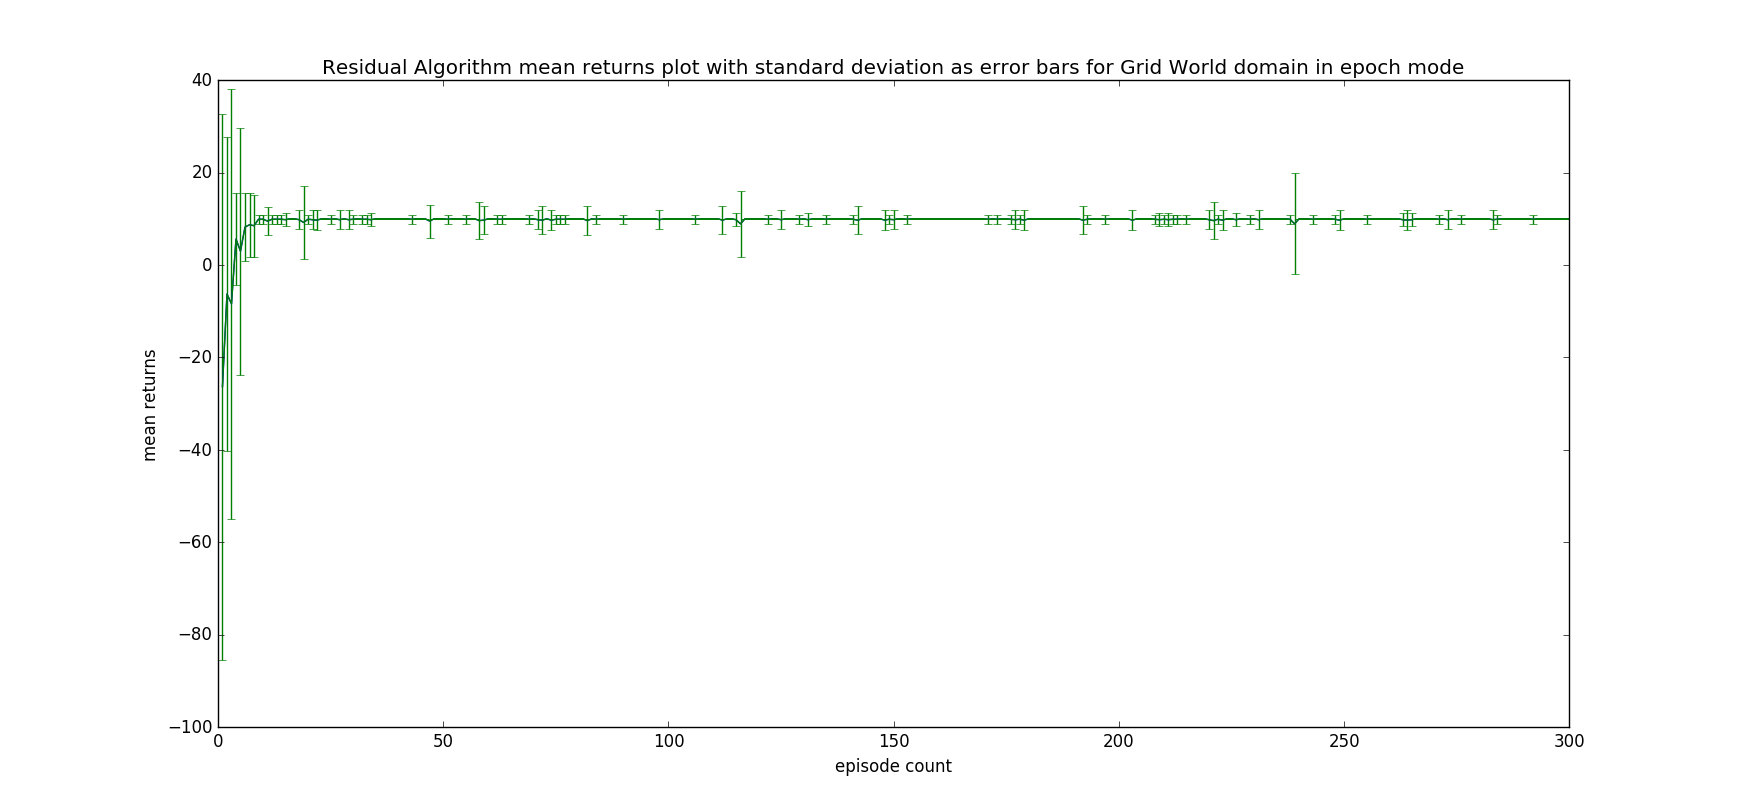
\includegraphics[width=12cm]{gridworld_epoch_direct_grad.png} }}%
    \qquad
    \subfloat[$\phi =1$]{{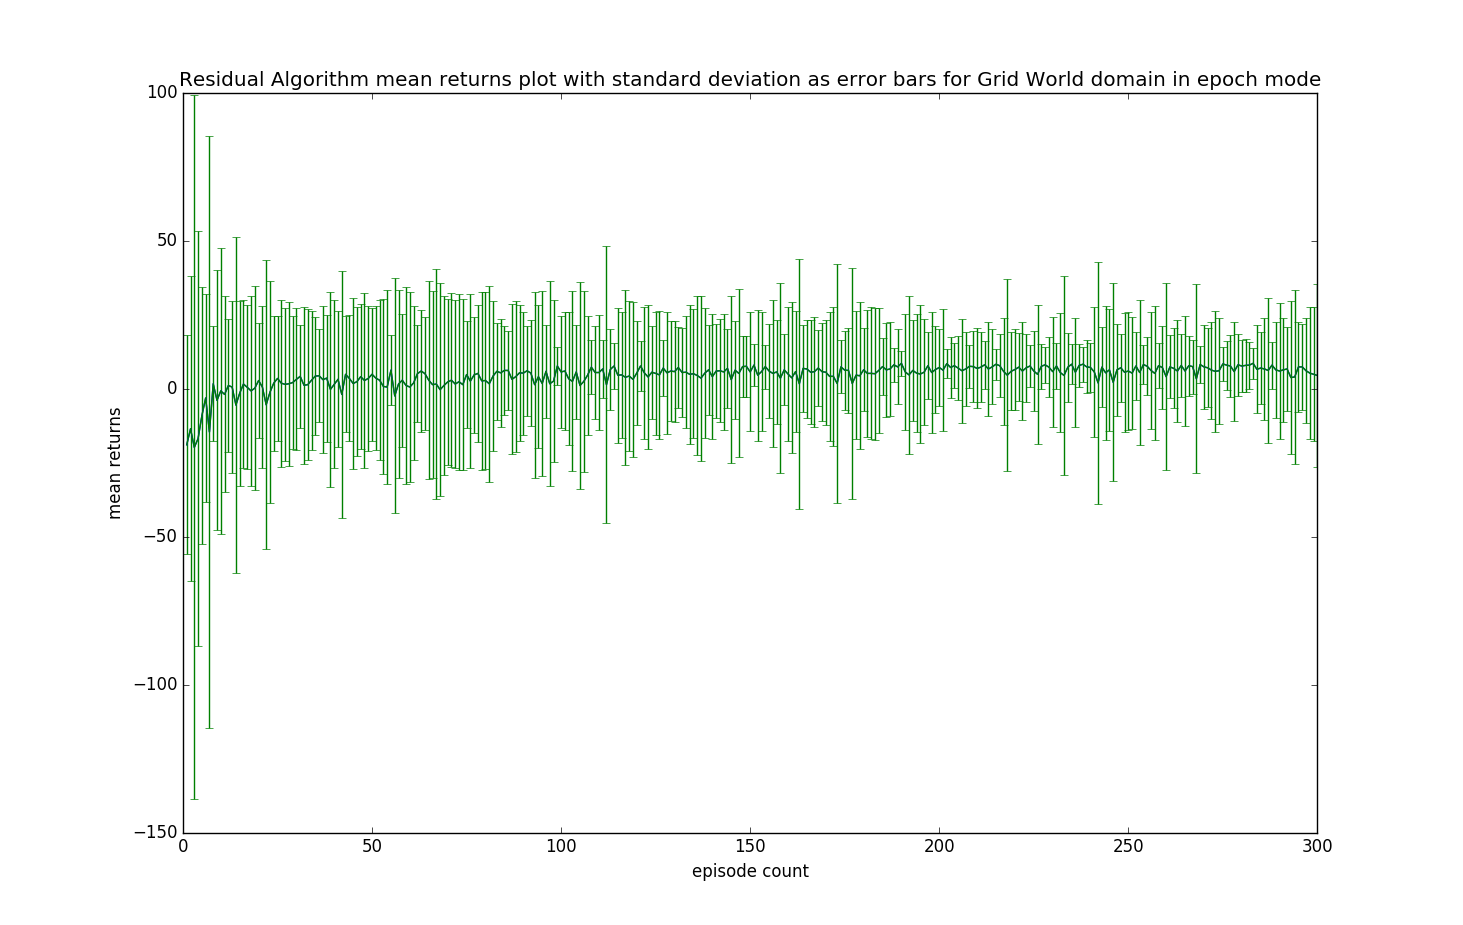
\includegraphics[width=12cm]{gridworld_epoch_residual_grad.png} }}%
    \qquad
    \subfloat[Adaptive $\phi$]{{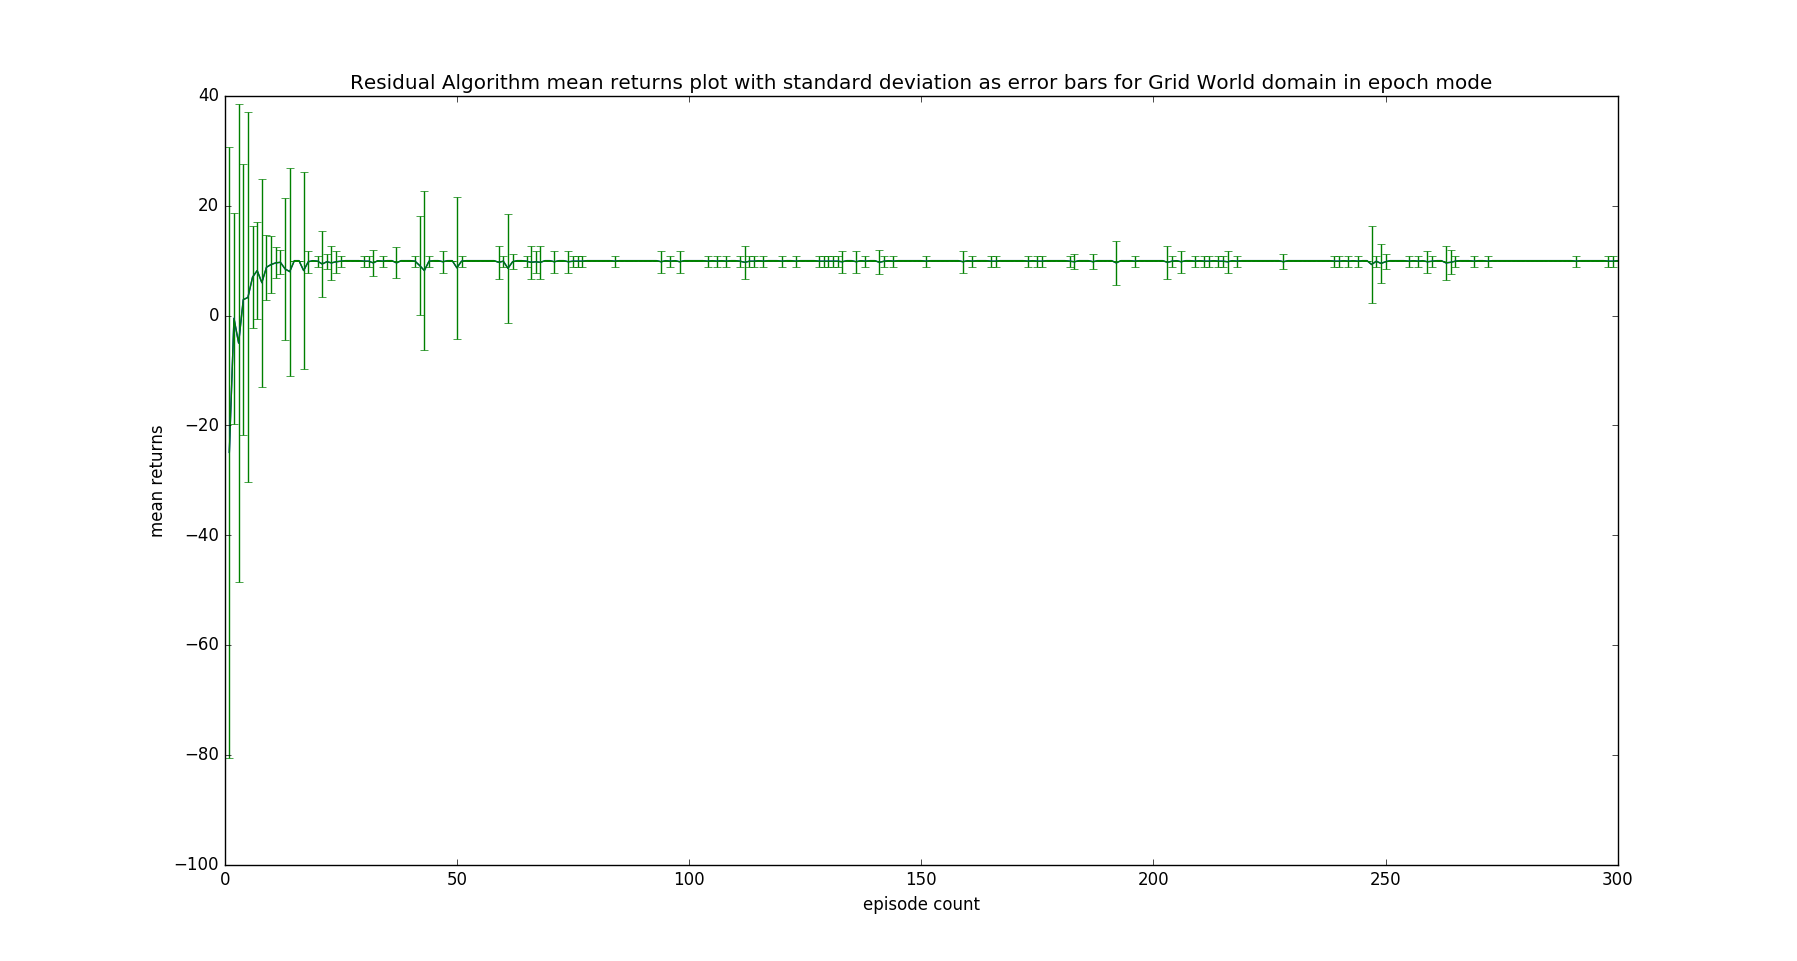
\includegraphics[width=12cm]{gridworld_epoch_adaptive.png} }}%
    \caption{Mean Returns Vs Episodes plot in epoch training mode for Grid World}%
    \label{fig:example}%
\end{figure}

\begin{figure}%
    \centering
    \subfloat[$\phi = 0$]{{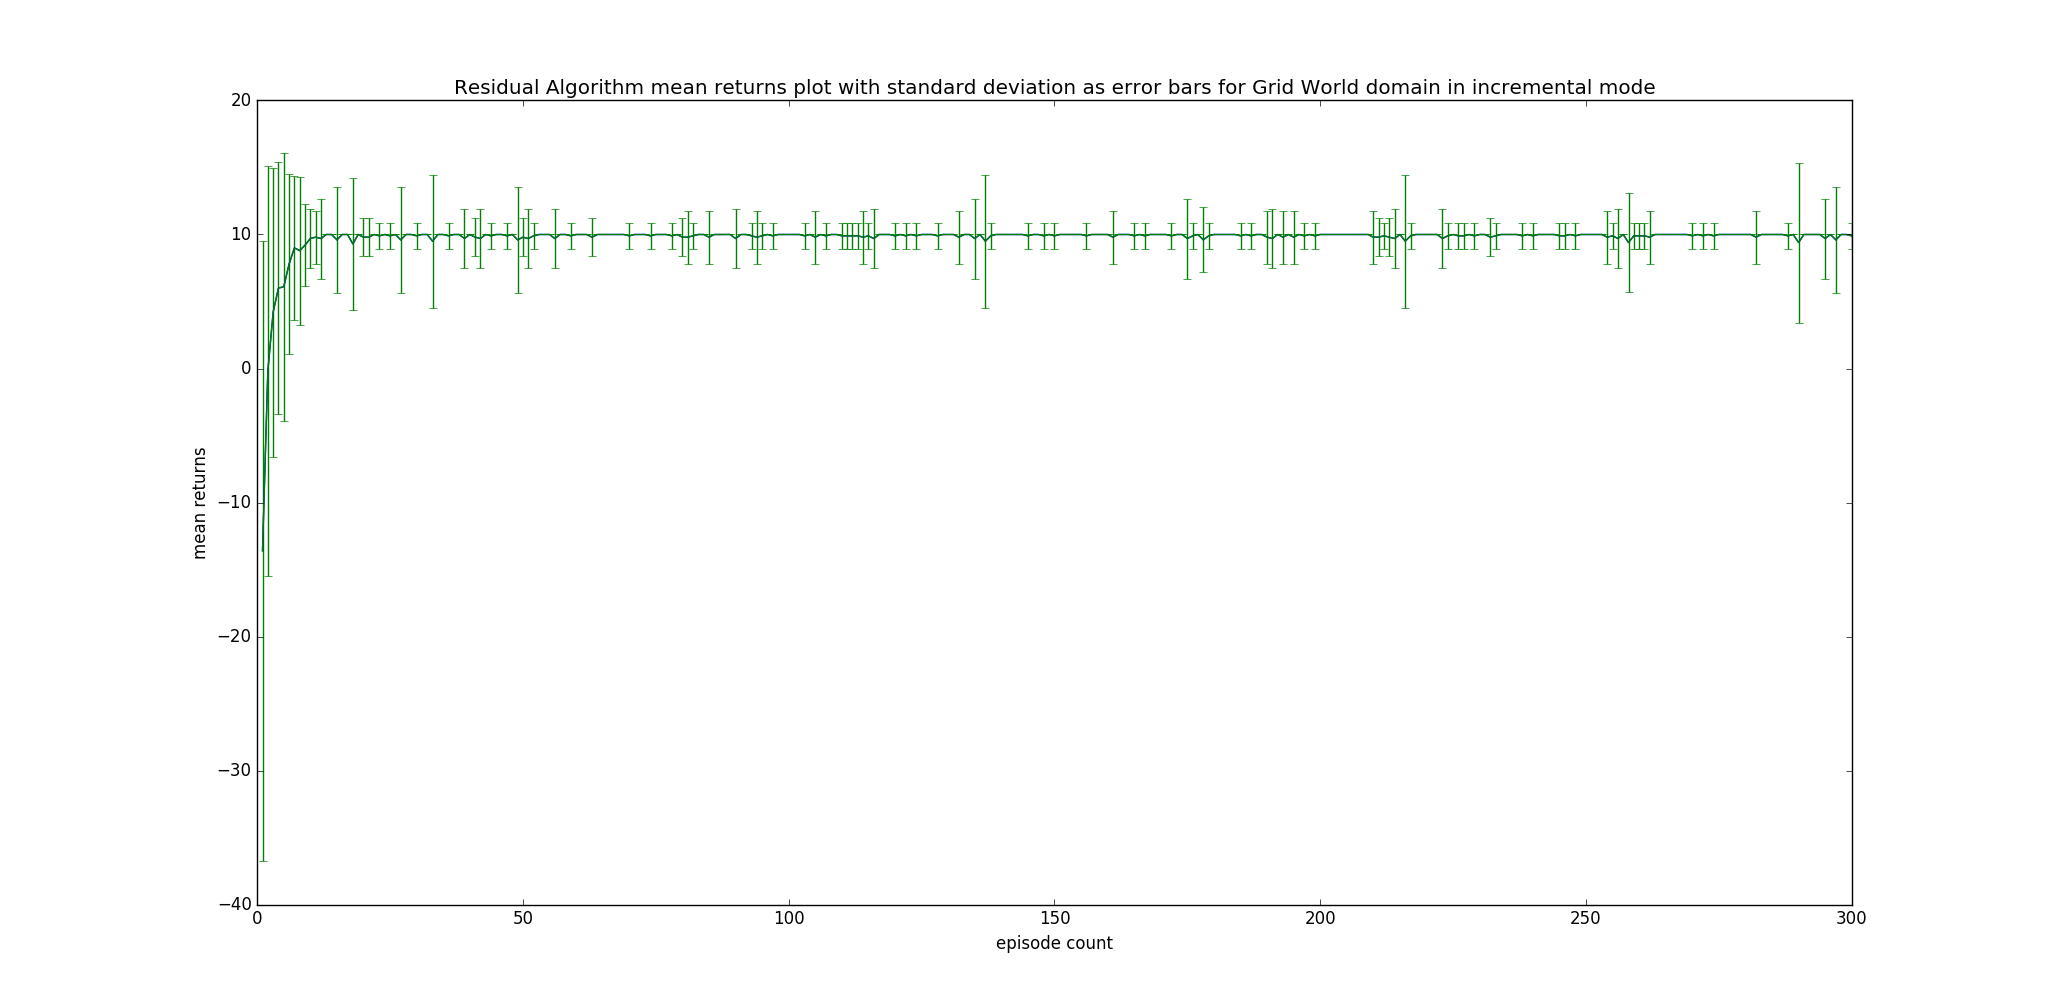
\includegraphics[width=12cm]{gridworld_incremental_direct_grad.png} }}%
    \qquad
    \subfloat[$\phi =1$]{{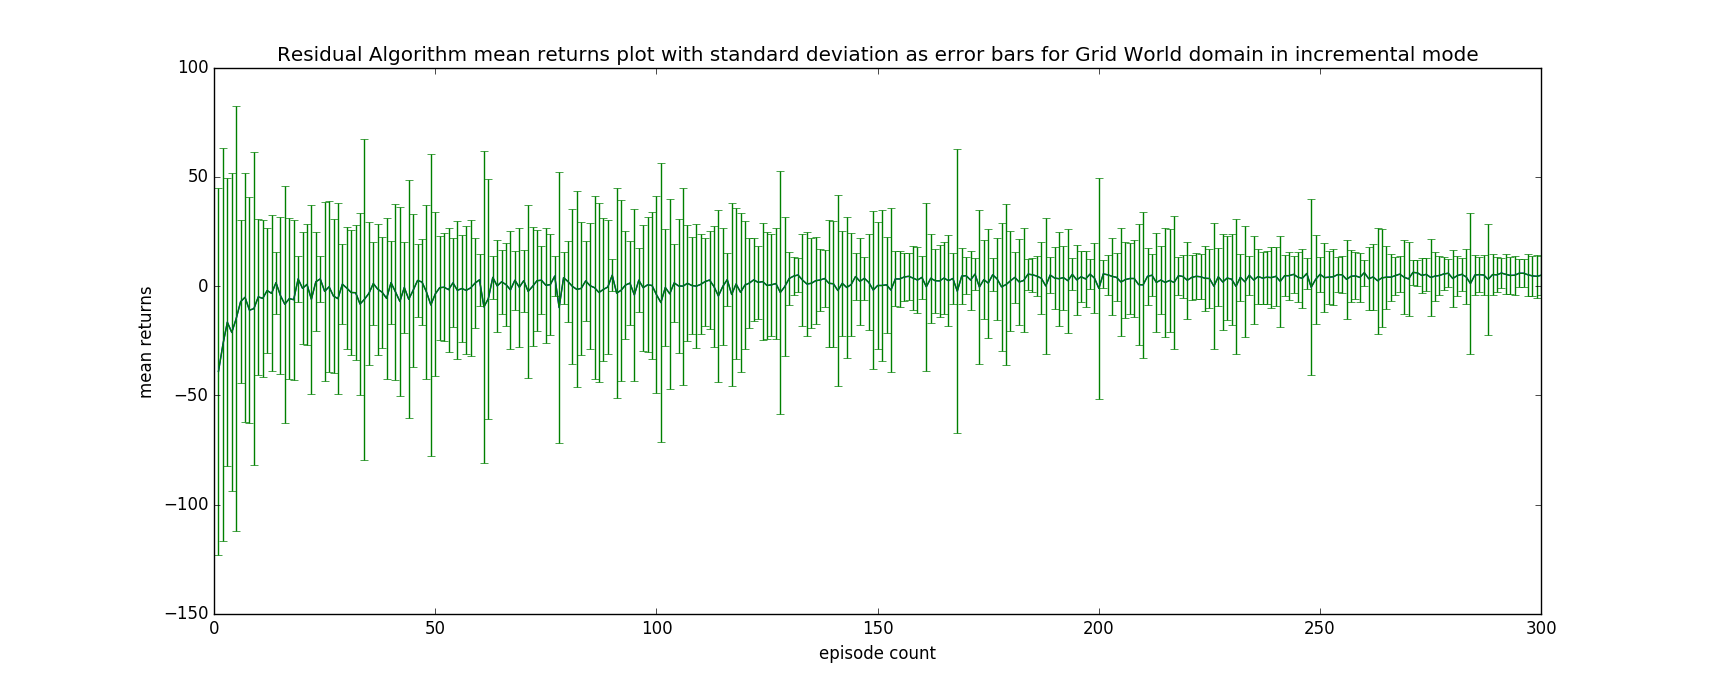
\includegraphics[width=12cm]{gridworld_incremental_residual_grad.png} }}%
    \qquad
    \subfloat[Adaptive $\phi$]{{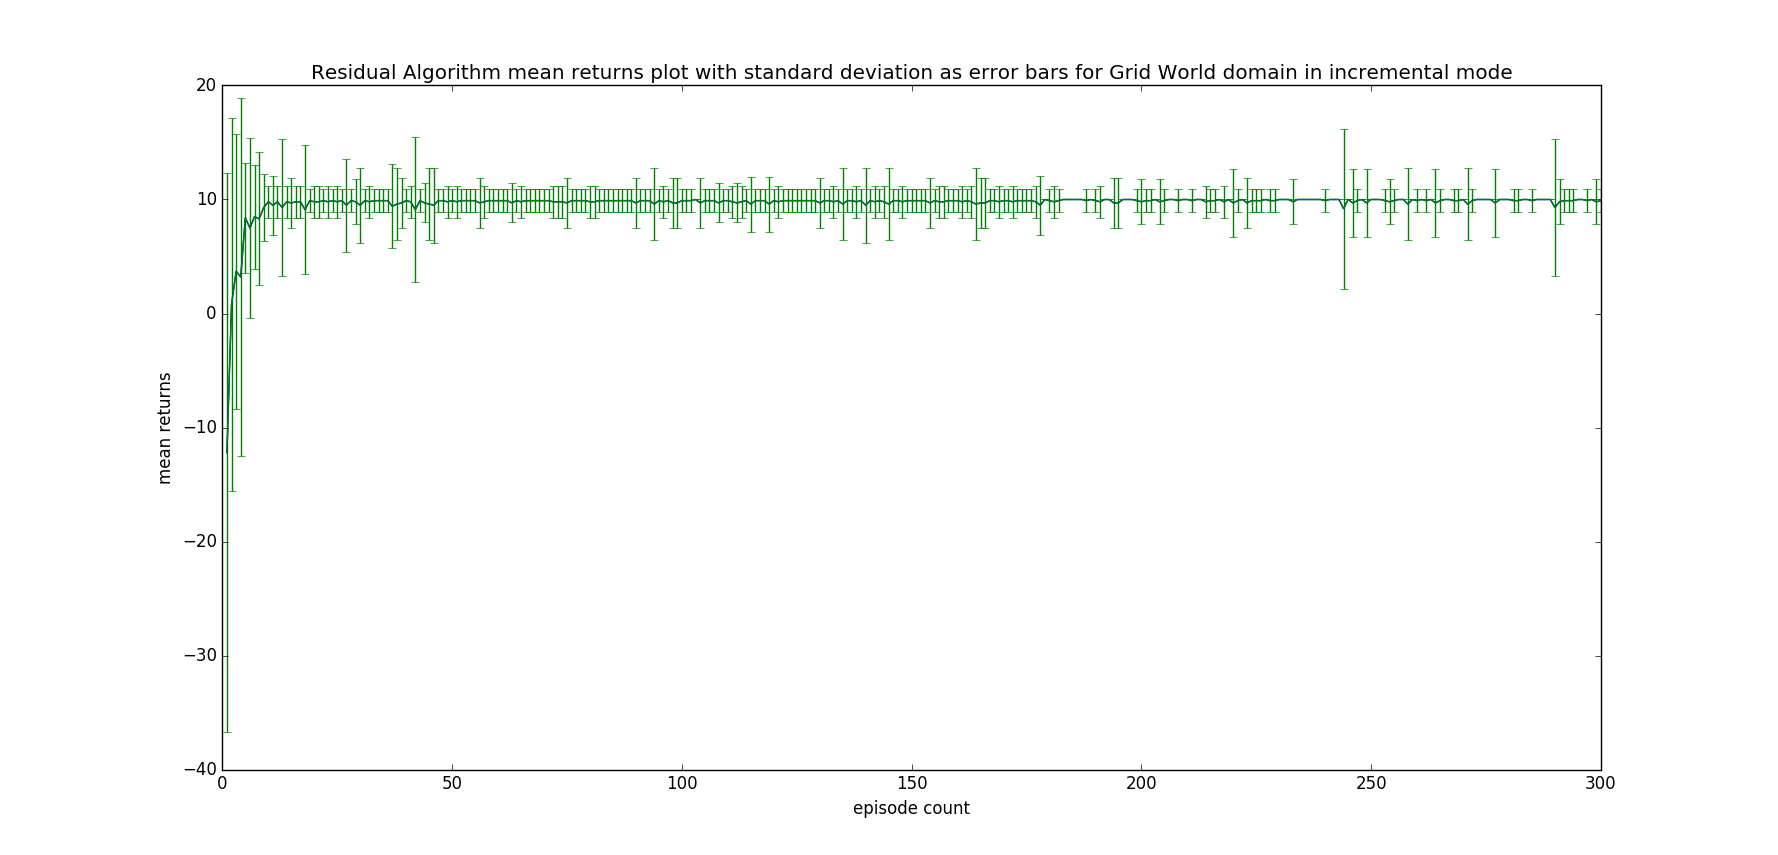
\includegraphics[width=12cm]{gridworld_incremental_adaptive.png} }}%
    \caption{Mean Returns Vs Episodes plot in incremental training mode for Grid World}%
    \label{fig:example}%
\end{figure}



\begin{figure}%
\begin{center}
\begin{tabular}{ |c|c|c|c| } 
 \hline
           & Epoch Mode & Incremental Mode \\
 $phi = 0$ & 52.19 & 57.51 \\ 
 $phi = 1$ & 1046.95 & 2339.006 \\ 
 Adaptive $\phi$ & 63.78 & 120.22 \\ 
 \hline
\end{tabular}
\end{center}
\caption{Running times for Grid World in seconds}%
    \label{fig:example}%
\end{figure}




\subsection*{Results for the Mountain Car}

The following hyperparameters were used to train the algorithm on Grid World:
TRIALS COUNT = 100, EPISODE COUNT = 300, MAX TIME STEP = 2000, ALPHA = 0.03, MU = 0.05, FOURIER ORDER = 1, EPSILON = 0.05 (for $\epsilon$ greedy exploration) and GAMMA = 1.

The hyperparameters were tuned manually by altering the values of GAMMA, EPSILON, FOURIER ORDER and ALPHA to obtain the best mean rewards.

In fig 5, we can observe the mean rewards obtained on mountain car in the epoch training mode. Similarly fig 6 provides the mean rewards plot in the incremental training mode. We can observe that in each of the training modes the the direct algorithm and the residual algorithm are able to achieve the maximum reward while the residual gradient struggles and the rate of learning is really slow compared to the other models. In fig 4, we can observe that the algorithm learns faster in the incremental training mode compared to the epoch training mode and the training time of the residual algorithm is second to the direct algorithm methods.
\begin{figure}%
\begin{center}
\begin{tabular}{ |c|c|c|c| } 
 \hline
           & Epoch Mode & Incremental Mode \\
 $phi = 0$ & 572 & 398.98 \\ 
 $phi = 1$ & 7829.71 & 4914.646 \\ 
 Adaptive $\phi$ & 588.56 & 480.447 \\ 
 \hline
\end{tabular}
\end{center}
\caption{Running times for Mountain Car in seconds}%
    \label{fig:example}%
\end{figure}

\begin{figure}%
    \centering
    \subfloat[$\phi = 0$]{{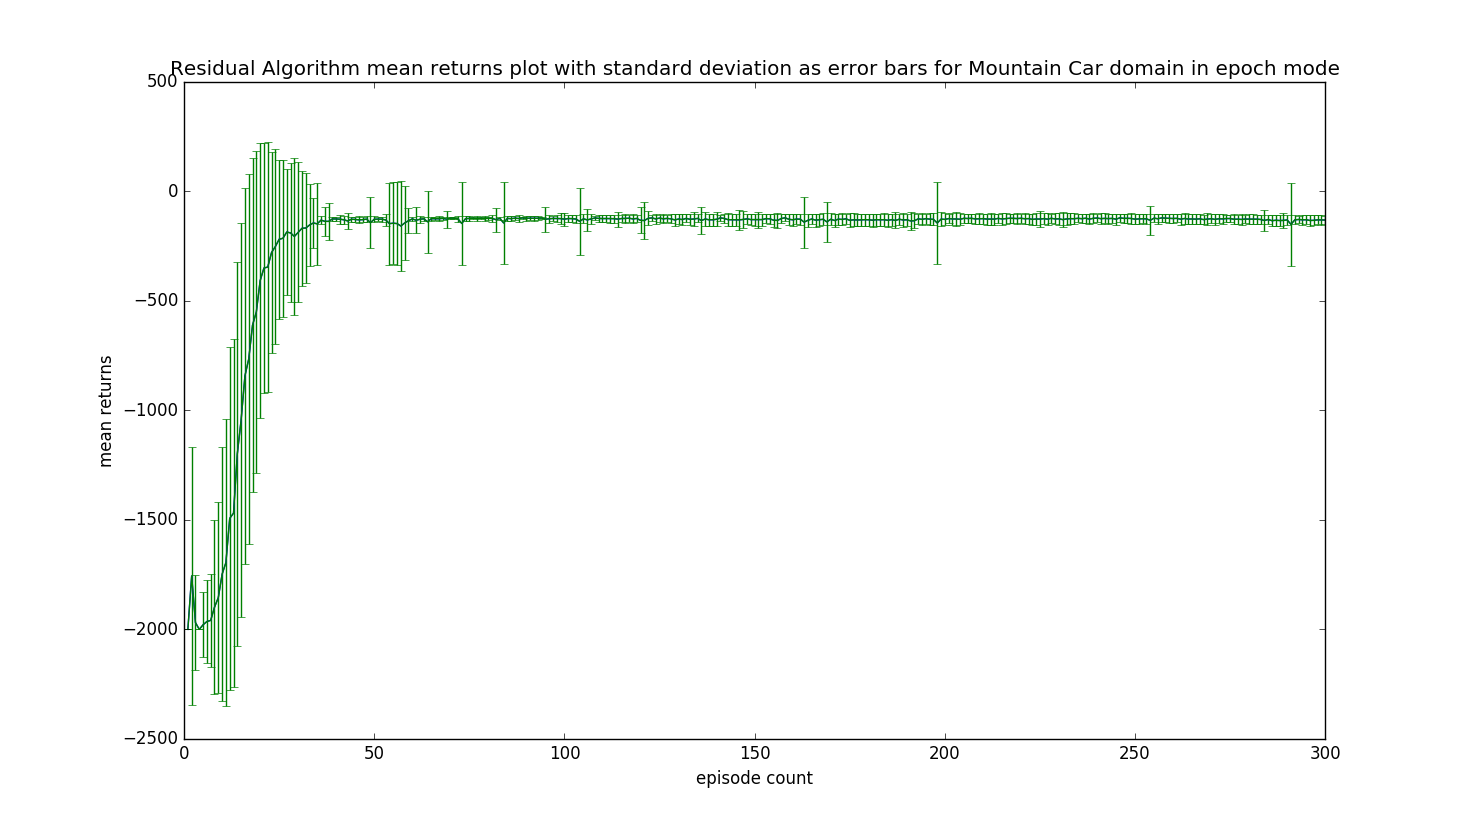
\includegraphics[width=12cm]{mountain_car_epoch_direct_grad.png} }}%
    \qquad
    \subfloat[$\phi =1$]{{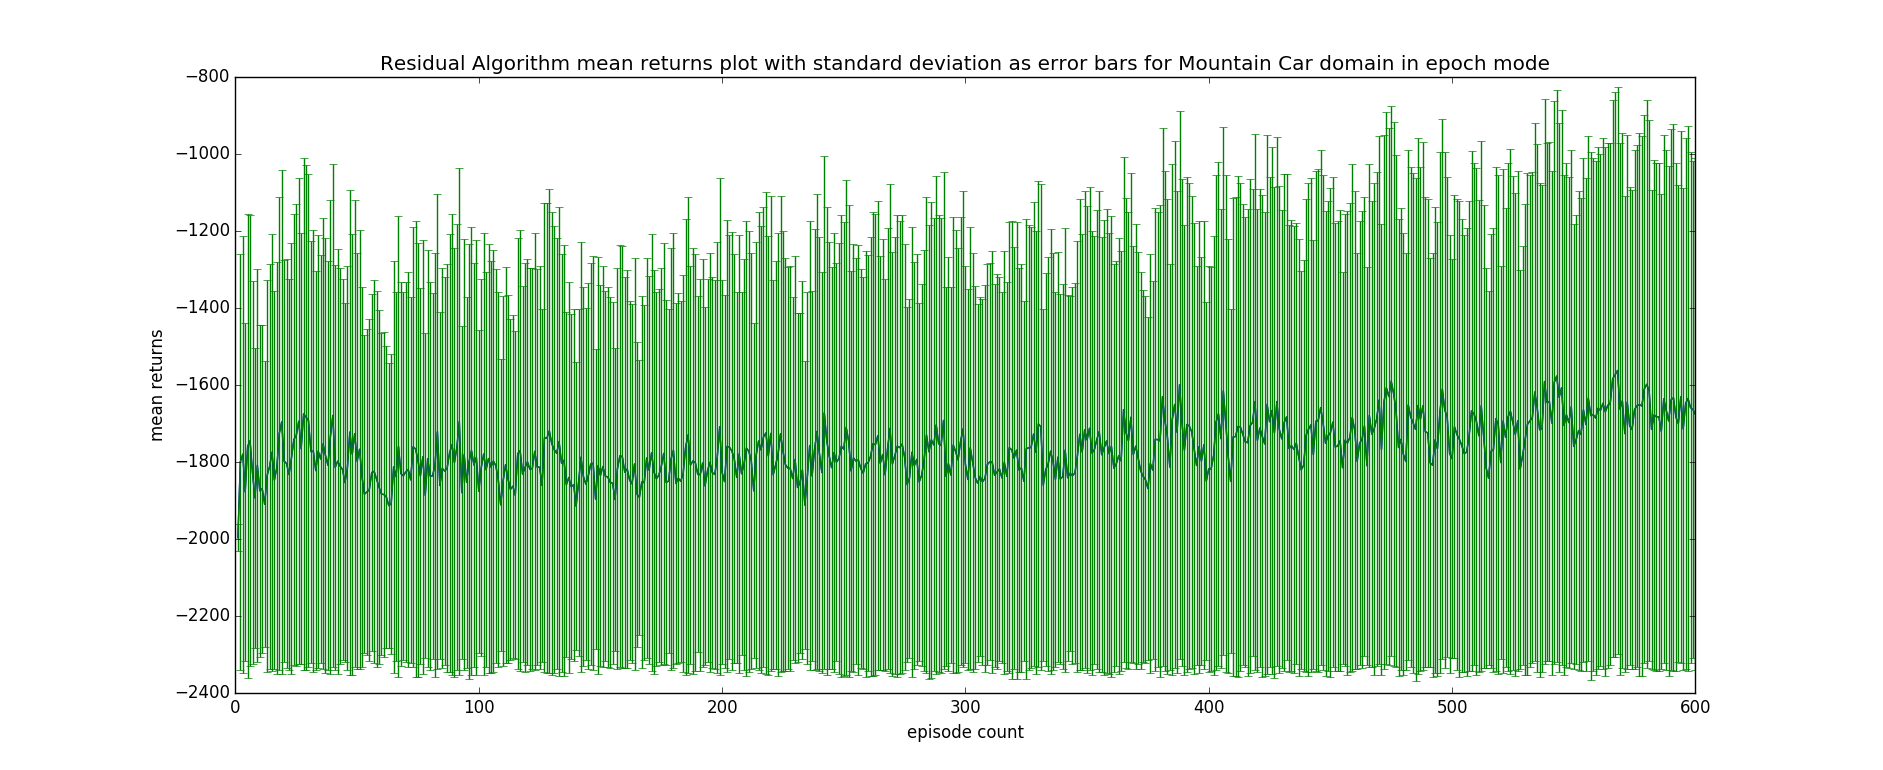
\includegraphics[width=12cm]{mountain_car_epoch_residual_grad.png} }}%
    \qquad
    \subfloat[Adaptive $\phi$]{{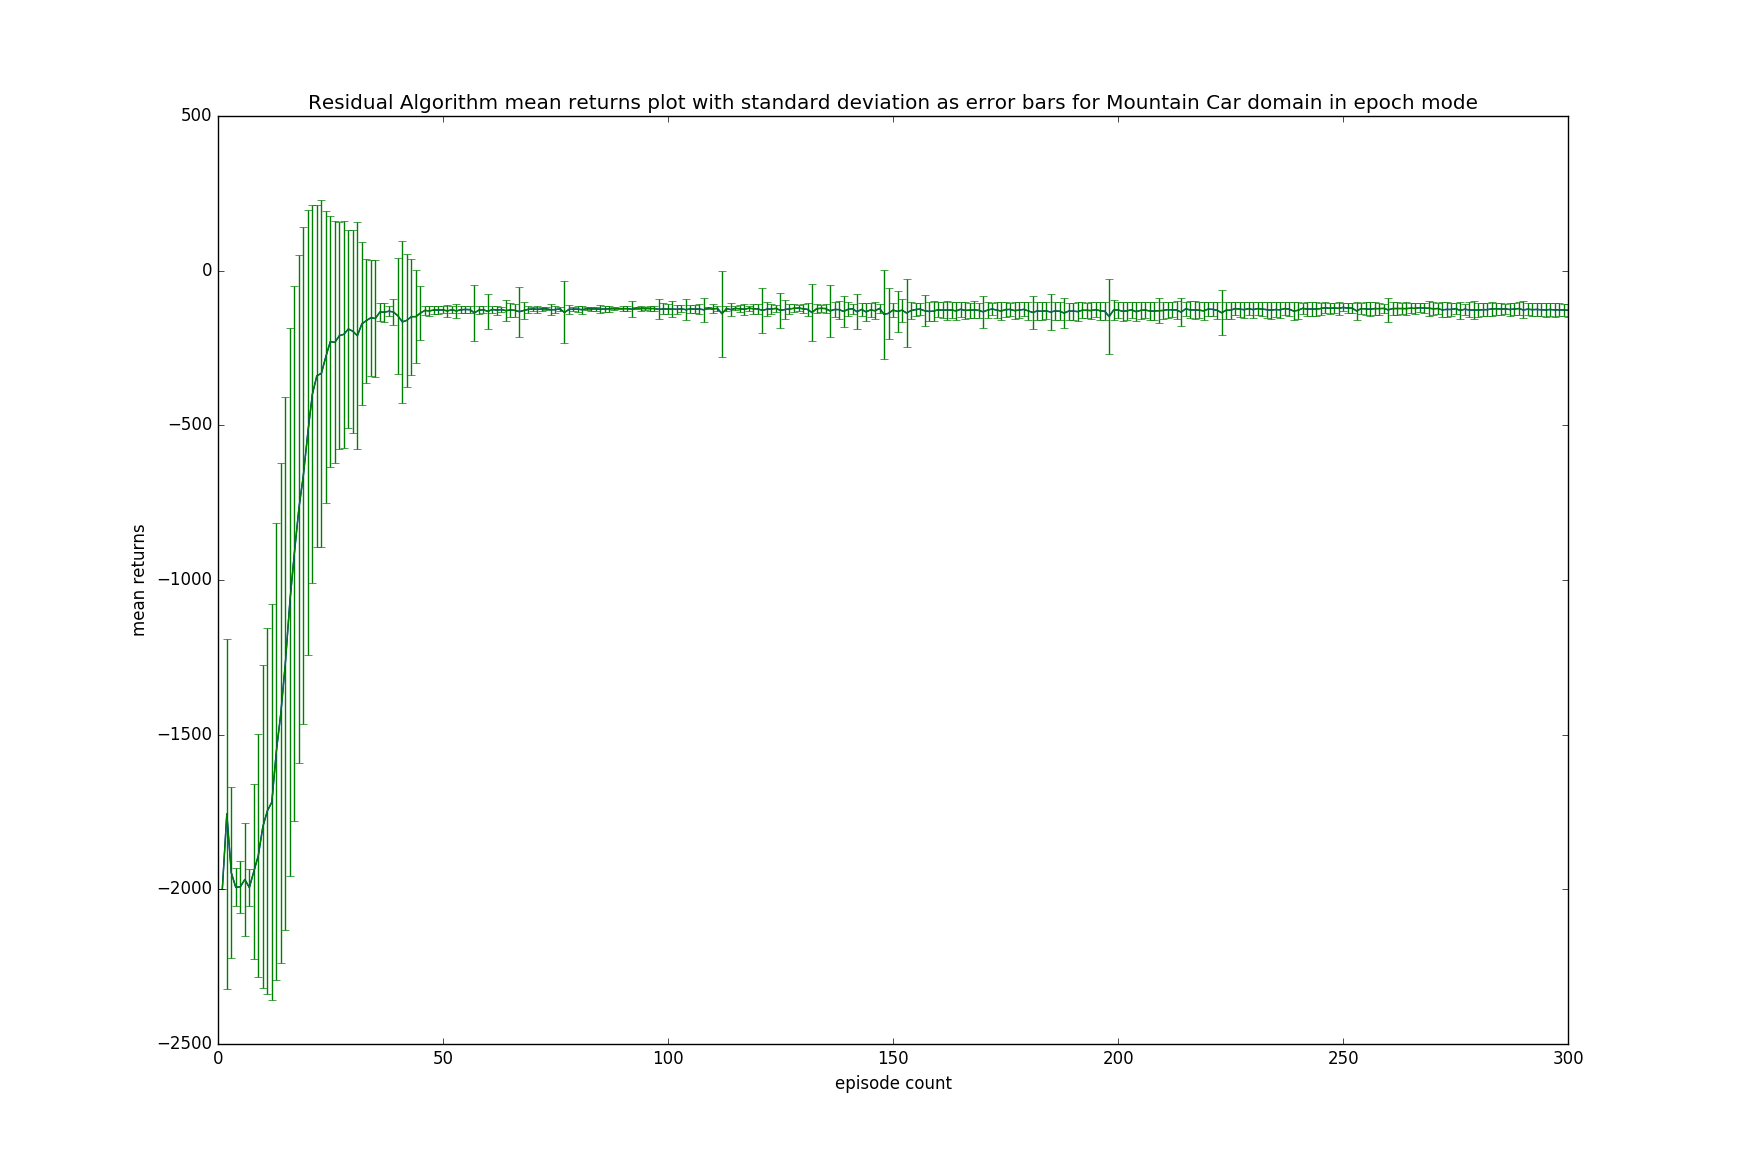
\includegraphics[width=12cm]{mountain_car_epoch_adaptive.png} }}%
    \caption{Mean Returns Vs Episodes plot in epoch training mode for Mountain Car}%
    \label{fig:example}%
\end{figure}

\begin{figure}%
    \centering
    \subfloat[$\phi = 0$]{{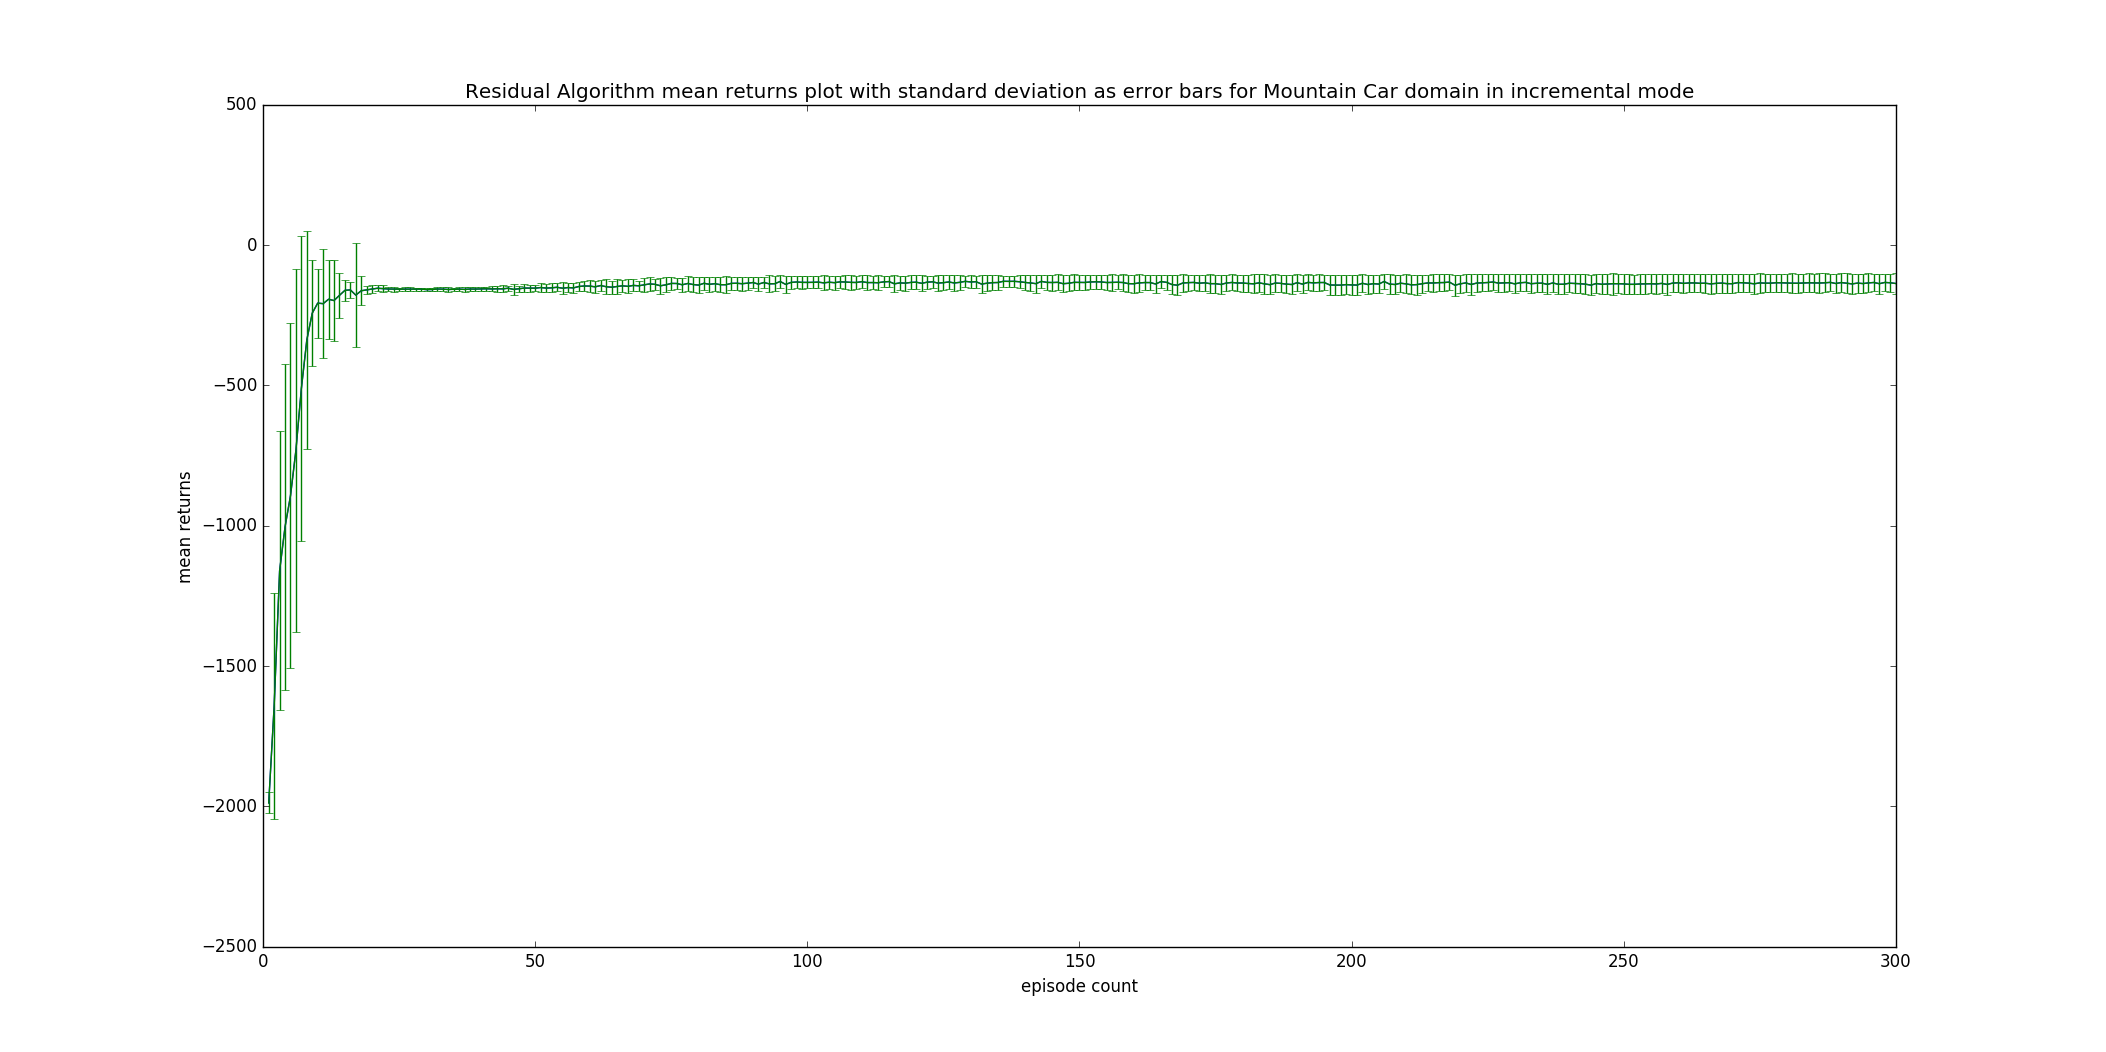
\includegraphics[width=12cm]{mountain_car_incremental_direct_grad.png} }}%
    \qquad
    \subfloat[$\phi =1$]{{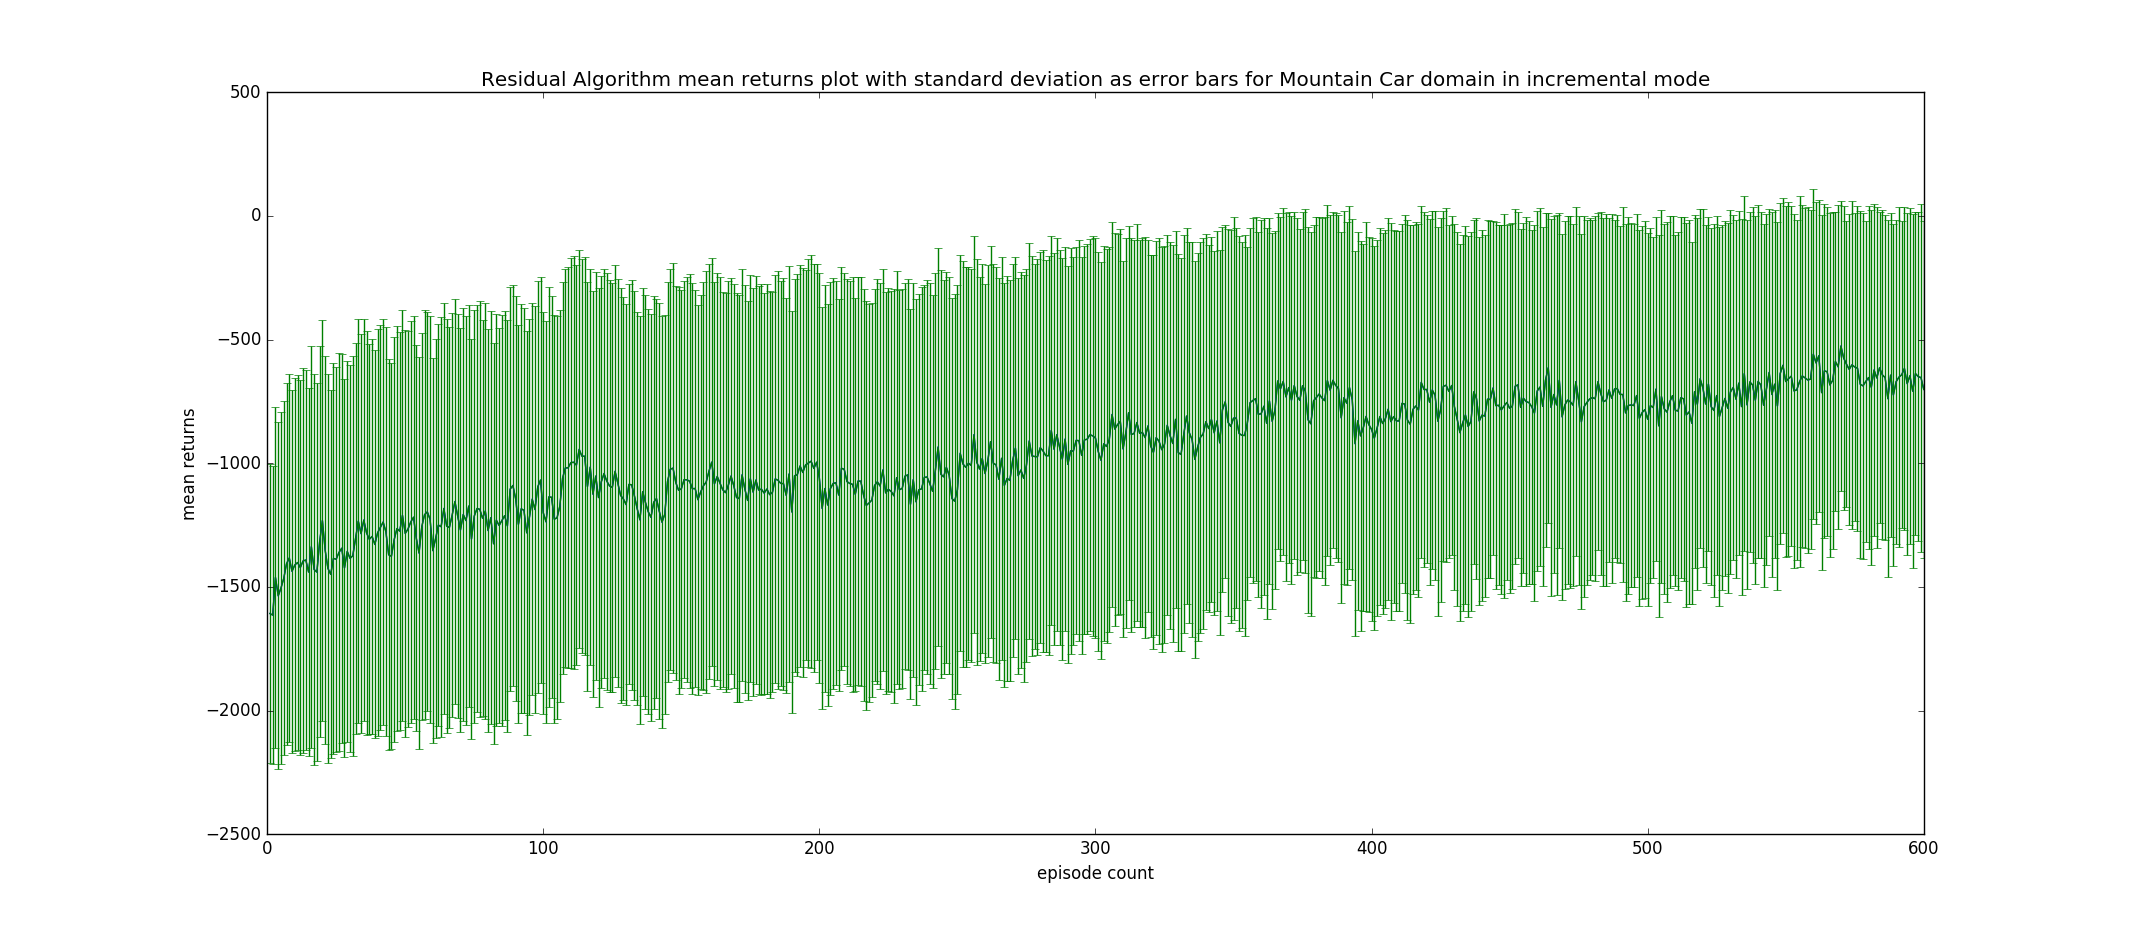
\includegraphics[width=12cm]{mountain_car_incremental_residual_grad.png} }}%
    \qquad
    \subfloat[Adaptive $\phi$]{{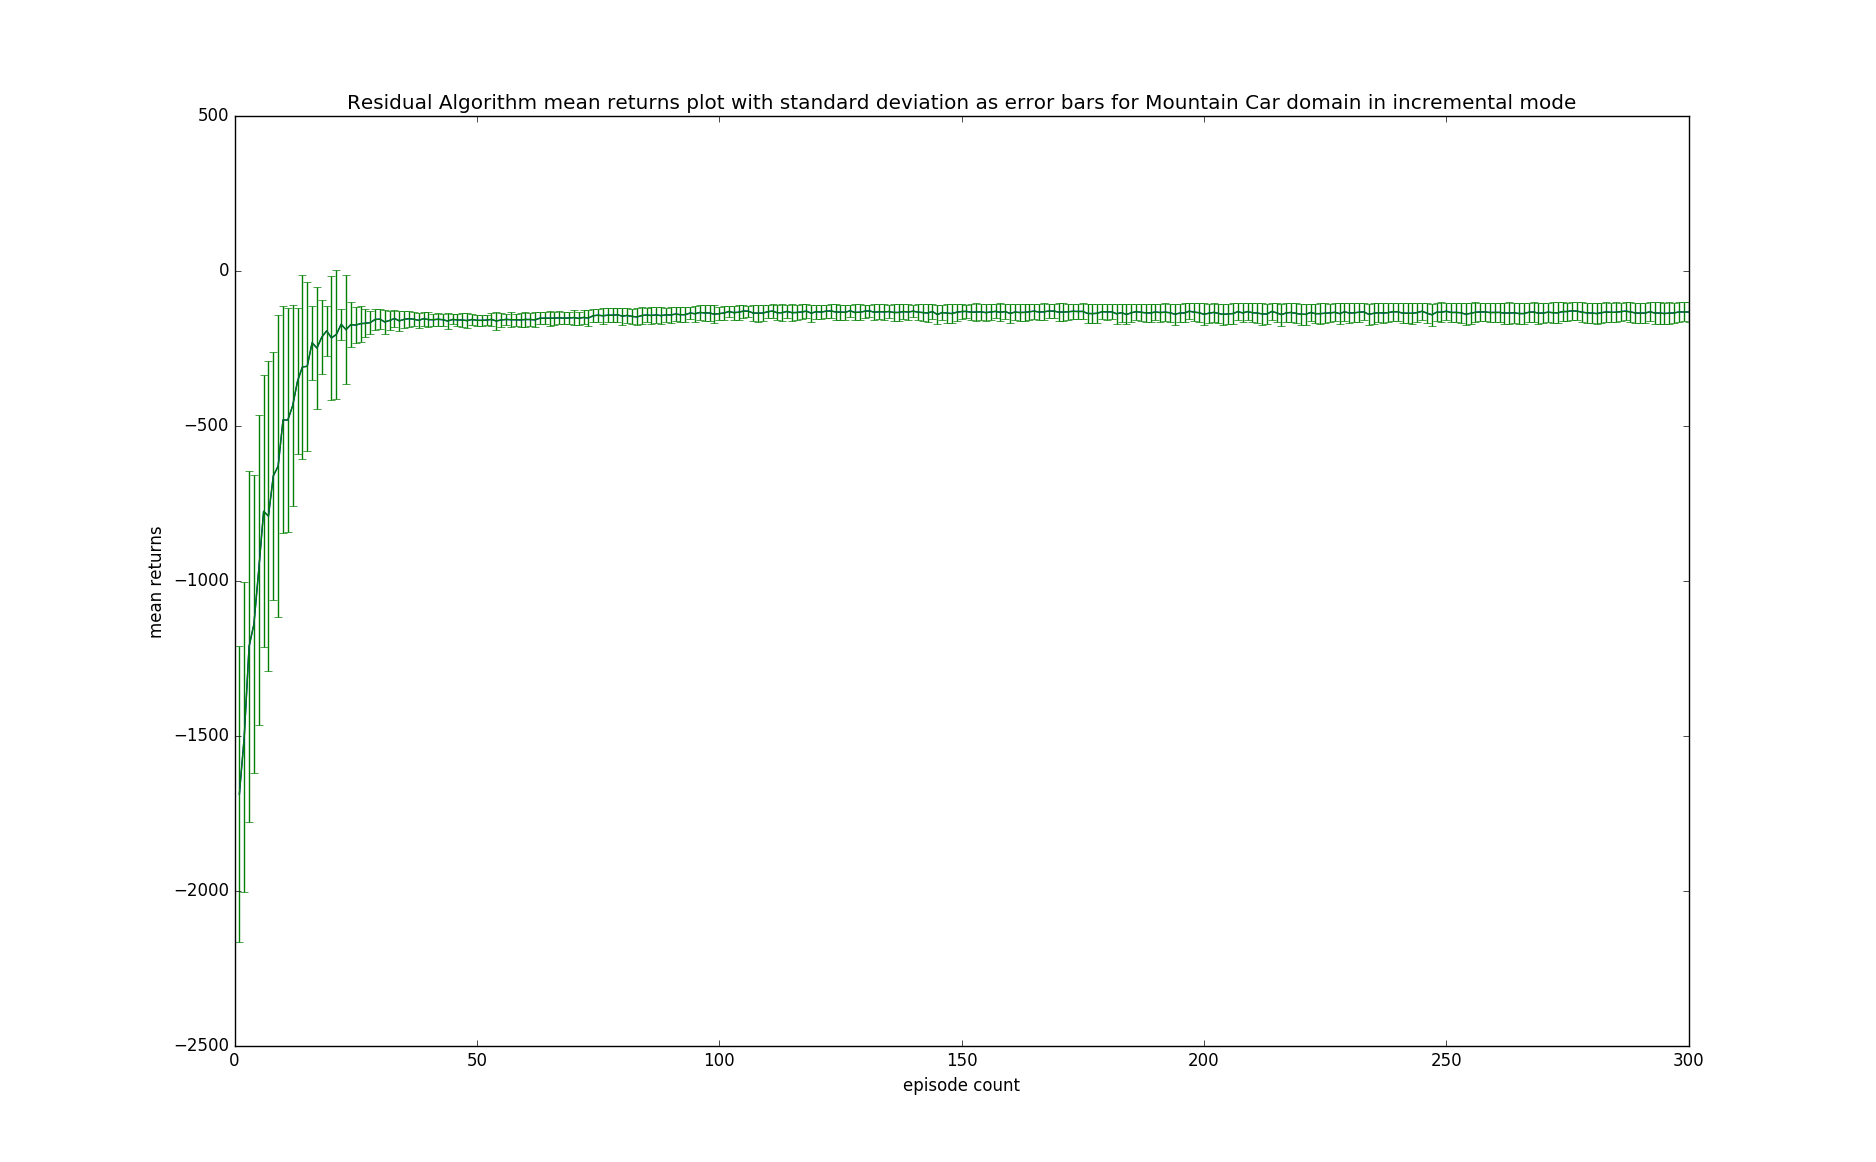
\includegraphics[width=12cm]{mountain_car_incremental_adaptive.png} }}%
    \caption{Mean Returns Vs Episodes plot in incremental training mode for Mountain Car}%
    \label{fig:example}%
\end{figure}

\end{document}
